De nos jours, les graphes sont omniprésents. Cependant, leur taille présentent un obstacle presque insurmontable à la compréhension du caractère essentiel des données. D'où la nécessité de la compression qui permet de réduire la taille des graphes tout en gardant le caractère utile de l'information incluse dans ces derniers.

Nous avons étudié dans ce chapitre différentes méthodes de compression de graphes dans le but d'établir une classification des méthodes basée sur deux approches : l'extraction de motifs et les arbres k2-trees. Nous nous sommes appuyer pour cela sur le principe de fonctionnement de chacune d'elles. Nous  proposons six classes de méthodes :

\begin{enumerate}[label=\roman*]
\item  Les méthodes de compression par les k2-trees
	\item  Les méthodes de compression par extraction de motifs basées vocabulaires en utilisant des méthodes de clustering.
	\item  Les méthodes de compression par extraction de motifs basées vocabulaires exploitant les propriétés de la matrice d'adjacence.
	\item  Les méthodes de compression par extraction de motifs basées agrégation de nœuds.
	\item  Les méthodes de compression par extraction de motifs basées agrégation de liens en utilisant des règles de grammaire.
	\item  Les méthodes de compression par extraction de motifs basées agrégation de liens en utilisant des heuristiques de clustering.
\end{enumerate}
	
Nous avons présenté le principe de fonctionnement des méthodes relatif à chaque classe tout en comparant leurs caractéristiques. 
 Ces classes diffèrent les unes des autres dans leurs fondements théoriques, le type de compression considéré, la complexité des algorithmes, les objectifs et les domaines d'application. 
 Dans le tableau \ref{comgen} , nous allons essayer de synthétiser les principales différences et similitudes entre les deux approches, compression par extraction de motifs et compression par les arbres k2-trees, que nous avons pu constater à travers notre recherche bibliographique. Ils ont un fort impact sur le choix de la méthode de compression du moment qu'ils ont une influence directe sur les performances.
 
\begin{table}[H]
\begin{tabular}{|c|p{6cm}|p{4cm}|}

\hline & \begin{center}
\textbf{$k^2$-trees}
\end{center}     &  \begin{center} \textbf{Extraction de motifs} \end{center}  \\
										
										
\hline Type de compression & toujours sans perte & toujours sans perte \\
\hline Structure en sortie & Toujours succincte & Peut être succincte où structurelle où les deux en même temps\\

\hline technique utilisée & exploitation de la matrice d'adjacence du graphe & exploitation des motifs fréquents dans le graphe\\

\hline Dépendance & Dépend du paramètre k & Dépend selon la méthode de l'algorithme de clustering ou du vocabulaire de motifs utilisé  \\

\hline Objectif & 
\begin{minipage}[t]{0.35\textwidth}
  			Compression,\\
  			Réduire l'espace de stockage et le temps de parcours\\
  \end{minipage}
  &
  \begin{minipage}[t]{0.25\textwidth}
  			- Compression,\\
  			- Réduire l'espace de  stockage et le temps de parcours,\\
  			- Extraire les informations pertinentes, \\
  			- Visualisation \\
  \end{minipage}
  \\
  \hline Domaine d'application & tous les domaines & tous les domaines \\
  \hline Type de graphes supporté & 
 \begin{minipage}[t]{0.25\textwidth}
  			- Statique orienté,\\
  			- Attribué,\\
  			- Dynamique, \\
  \end{minipage}  
  &  \begin{minipage}[t]{0.25\textwidth}
  			- Statique (orienté et non orienté),\\
  			- étiqueté,\\
  			- Dynamique, \\
  \end{minipage}  
  \\ \hline
\end{tabular}
									\caption{Comparaison entre les méthodes basées sur$k^2$-trees et basées sur l'extraction de motifs.}									\label{comgen}
									
								\end{table}
								
				
				
				Après avoir comparer les caractéristiques des deux classes de méthodes de compression, nous sommes intéressées à comparer les résultats expérimentales obtenues dans leur différents travaux et utilisant les même graphes de test. À ce stade, notre but est d'établir une étude comparative plus approfondie sur les performances des deux classes. Les deux courbes de la figure \ref{comparaisonVo} présentent le nombre de bits par liens obtenues sur deux graphes de test uk-2002 et eu-2005 (Nous fournissons plus de détails sur ses deux graphes en annexe \ref{tableau_test}).
				
				D'après la figure, on constate que les deux courbes atteignent leur minimum dans le cas de la méthode DSM \citep{hernandez2014compressed} avec 2,11 (bpe) pour eu-2005 et 1,53 (bpe) pour uk-2002. Cette méthode donne ainsi le meilleur résultat dans les deux classes. 	
Nous remarquons aussi que les méthodes basées vocabulaire en utilisant les propriétés de la matrice d'adjacence et la méthode de compression VNM \citep{buehrer2008scalable} s'inscrivant dans les méthodes de compression basées agrégation des liens des motifs usant des méthodes de clustering donnent des résultats presque équivalent aux deux méthodes de compression par les arbres $k^2$-trees: $k^2$-trees : Amélioration \citep{brisaboa2014compact} et Delta-$k^2$-trees  \citep{zhang2014delta}. D'autre part, la première méthode \citep{claude2010fast} des méthodes de compression par extraction de motifs  basées agrégation de liens des motifs en utilisant des règles de grammaire donne le même nombre de bits que l'algorithme de base k2-trees \citep{brisaboa2009k}. Tant dis que la deuxième méthode \citep{claude2010extended} de cette même classe améliore de manière significative le résultat donnant ainsi de meilleurs performances.

\begin{figure}[H]	
				\centering						
				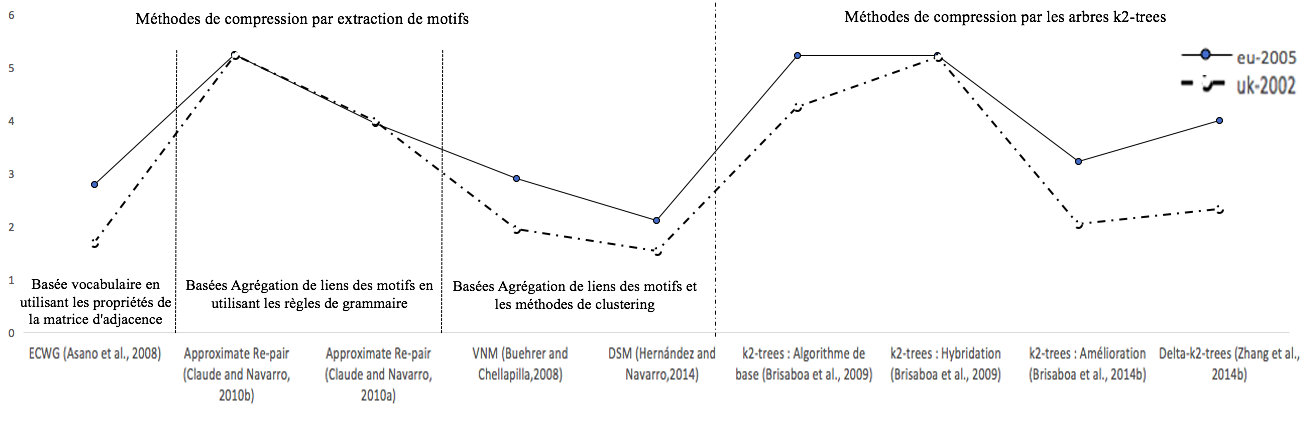
\includegraphics[scale=0.38]{ressources/image/globale.png} 
					\centering
					\caption{Comparaison des performances des méthodes par extraction de motifs et les méthodes basées sur les arbres $k^2$-trees }
					\label{comparaisonVo}
				\end{figure}				
				
				
				
								
								Nous avons aussi constaté que malgré le nombre considérable de travaux dans
le domaine de la compression des graphes, il y a encore
de nombreux problèmes ouverts importants sur le terrain. Nous mentionnons ci-dessous quelques un des plus remarquables.
 

Le premier est l'aspect récursive des méthodes de construction des arbres k2-trees qui est un obstacle envers les performances (complexité temporelle et spaciale) de cette classe de méthodes. Certe l'utilisation de l'approche récursive permet souvent d'avoir un programme naturel, plus simple et plus facile à comprendre mais le nombre important d'appels imbriqués générés dans le cas des graphes du monde réel augmente de manière considérable le temps d'exécution et la mémoire nécessaire pour la construction du graphe compressé. 

Le deuxième aspect est la forte influence des méthodes de clustering sur les performances de la compression. Certes, \gls{ConDenSe} améliore le taux de compression mais il détériore le taux d'exécution \citep{liu2018reducing}.

Un autre aspect à considérer est l'aspect temporel des graphes. En effet, tant dis que plusieurs méthodes de compression par les arbres k2-trees existent pour ce type de graphes, nous n'avons trouver que quelques méthodes dans le cas des méthodes par extraction de motifs basées vocabulaire et aucune méthodes dans la sous-classe des méthodes agrégatives malgré qu'elles offrent un taux de compression compétitif dans le cas statique. De plus, il existe peu de travaux sur la compression par les arbres k2-trees des graphes temporels attribués et aucun travail, à notre connaissance, sur la compression par extraction de motifs pour ce type de graphe. Cependant, de nombreux réseaux du monde réel, tels que les réseaux sociaux où le suivie des communautés (ou motifs) est très utile, peuvent facilement être modélisés sous la forme de graphes attribués temporels. Nous avons même remarqué que dans le cas de certains types de graphes statiques, tel que les graphes multi-vue, aucun schéma de compression n'a été proposé. Une solution dans le cas de l'exemple précédent serait peut être de généraliser le schéma de compression de VoG. Cette piste de recherche est motivé par l'apparition de nouvelles méthodes de clustering, comme celle proposée \citep{wang2019study}, adaptées pour les graphes multi-vue .


Finalement, nous pensons qu'une nouvelle direction prometteuse est l'utilisation des méthodes d'apprentissage dans le processus d'extraction de motifs des méthodes de compression. Le caractère prometteur de cette direction est due aux succès apporté par le domaine d'apprentissage ces dernières années, notamment le \textit{Deep Learning}. %De nombreux chercheurs se sont déjà investis dans le domaine, à l'exemple de \citep{sun2019big}.
								

